\documentclass[10pt,a4paper]{article}
\usepackage[utf8]{inputenc}
\usepackage[german]{babel}
\usepackage{mathrsfs}
\usepackage{amsmath}
\usepackage{amsfonts}
\usepackage{amssymb}
\usepackage{amsthm}
\usepackage{graphicx}
\usepackage{float}
\usepackage[left=2cm,right=2cm,top=2cm,bottom=2cm]{geometry}

\begin{document}

Stochastik 1, Blatt 5\\
Gruppe 1\\
Marten Lienen (2126759)\\
Fabian Schmittmann (2083559)

\section{Aufgabe 17}

\subsection{Teil a}

\subsection{Teil b}

\section{Aufgabe 18}

\begin{figure}[H]
  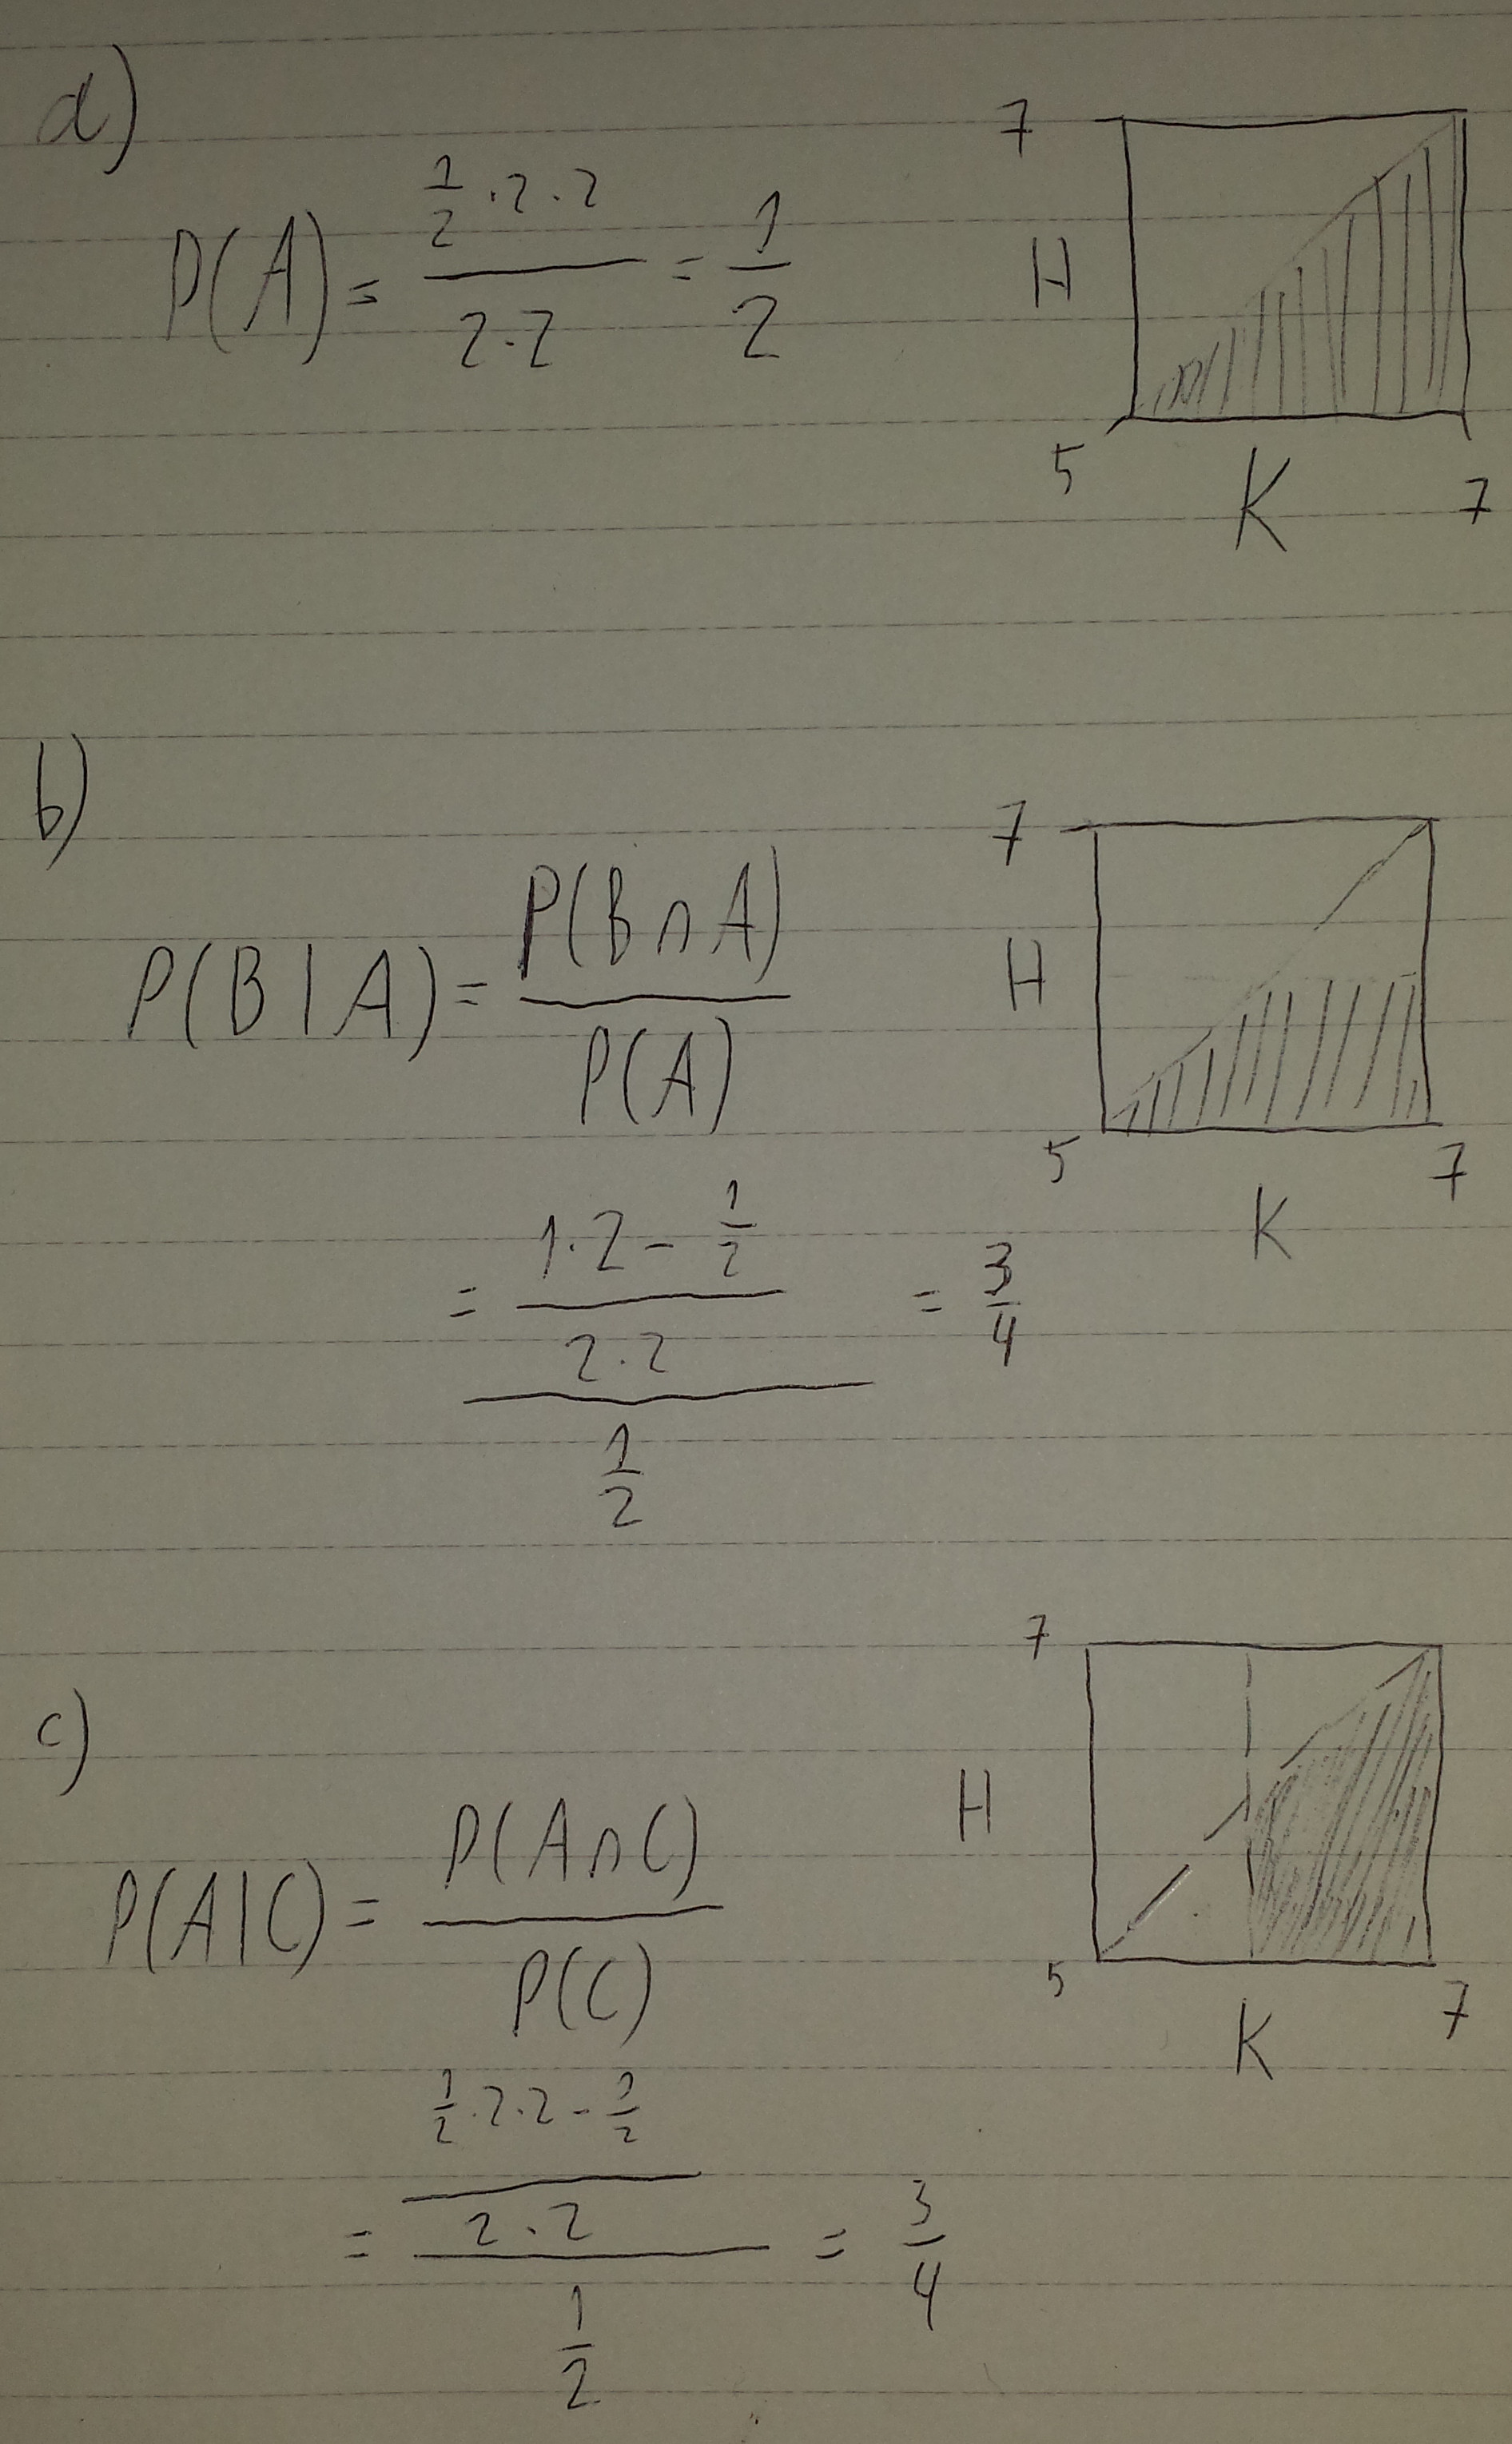
\includegraphics[width=400pt]{5_2}
\end{figure}

\subsection{Teil d}
\begin{equation}
  F(x) = 
  \begin{cases}
    0 & \textit{wenn $x < 0$}\\
    x & \textit{wenn $0 \le x \le 0.5$}\\
    0.5 + \frac{x - 0.5}{2} & \textit{wenn $0.5 < x \le 1.5$}\\
    1 & \textit{wenn $1.5 < x$}
  \end{cases}
\end{equation}

\section{Aufgabe 19}

\subsection{Teil a}
\begin{equation}
  F(x) = 
  \begin{cases}
    0 & \textit{wenn $x < a$}\\
    1 & \textit{wenn $x > b$}\\
    \frac{x - a}{b - a} & \textit{sonst}
  \end{cases}
\end{equation}

\subsection{Teil b}
\begin{align*}
  F(x) & = 
  \begin{cases}
    0 & \textit{wenn $x < 0$}\\
    \int_{a = 0}^{x} \lambda \cdot e^{-\lambda a} da & \textit{sonst}
  \end{cases}\\
  & = 
  \begin{cases}
    0 & \textit{wenn $x < 0$}\\
    1 - e^{-\lambda x} & \textit{sonst}
  \end{cases}
\end{align*}

\subsection{Teil c}
\begin{equation}
  F(x) = 
  \begin{cases}
    0 & \textit{wenn $x < 0$}\\
    1 - q^{\lfloor x \rfloor} & \textit{sonst}
  \end{cases}
\end{equation}

\subsection{Teil d}
Wenn $\alpha \ge 0$
\begin{equation}
  F(x) = F_{X}(\frac{x - \beta}{\alpha})
\end{equation}
Wenn $\alpha < 0$
\begin{equation}
  F(x) = 1 - \lim_{a \rightarrow x, a < x} F_{X}(\frac{a - \beta}{\alpha})
\end{equation}

\section{Aufgabe 20}

\end{document}